
%(BEGIN_QUESTION)
% Copyright 2007, Tony R. Kuphaldt, released under the Creative Commons Attribution License (v 1.0)
% This means you may do almost anything with this work of mine, so long as you give me proper credit

Suppose a voltmeter registers 6 volts between test points {\bf C} and {\bf D} while the pushbutton is released (not pressed), and also 6 volts between the same test points while the pushbutton is pressed:

$$\includegraphics[width=15.5cm]{i01861x01.eps}$$

Determine the diagnostic value of each of the following tests.  Assume only one fault in the system, including any single component or any single wire/cable/tube connecting components together.  If a proposed test could provide new information to help you identify the location and/or nature of the one fault, mark ``yes.''  Otherwise, if a proposed test would not reveal anything relevant to identifying the fault (already discernible from the measurements and symptoms given so far), mark ``no.''

% No blank lines allowed between lines of an \halign structure!
% I use comments (%) instead, so that TeX doesn't choke.

$$\vbox{\offinterlineskip
\halign{\strut
\vrule \quad\hfil # \ \hfil & 
\vrule \quad\hfil # \ \hfil & 
\vrule \quad\hfil # \ \hfil \vrule \cr
\noalign{\hrule}
%
% First row
{\bf Diagnostic test} & {\bf Yes} & {\bf No} \cr
%
\noalign{\hrule}
%
% Another row
Measure $V_{AB}$ with switch pressed &  &  \cr
%
\noalign{\hrule}
%
% Another row
Measure $V_{AC}$ with switch pressed &  &  \cr
%
\noalign{\hrule}
%
% Another row
Measure current through wire connecting {\bf B} to {\bf D} with switch pressed &  &  \cr
%
\noalign{\hrule}
%
% Another row
Measure $V_{AB}$ with switch unpressed &  &  \cr
%
\noalign{\hrule}
%
% Another row
Measure $V_{AC}$ with switch unpressed &  &  \cr
%
\noalign{\hrule}
%
% Another row
Measure $R_{EF}$ with switch pressed and source disconnected from {\bf E} &  &  \cr
%
\noalign{\hrule}
%
% Another row
Measure $R_{EF}$ with switch unpressed and source disconnected from {\bf E} &  &  \cr
%
\noalign{\hrule}
} % End of \halign 
}$$ % End of \vbox

\vfil 

\underbar{file i01861}
\eject
%(END_QUESTION)





%(BEGIN_ANSWER)

This is a graded question -- no answers or hints given!

%(END_ANSWER)





%(BEGIN_NOTES)

Note how the pushbutton's state is of no effect on the measured voltage, and how that voltage is precisely one-half that of the supply.  This suggests an ``open'' fault somewhere in the circuit branch containing $R_1$ and the pushbutton switch.  If we assume only component faults (not wiring faults between components), then the only two possibilities here are an open switch or an open $R_1$.

Any diagnostic test that would confirm either the switch or $R_1$ being failed open, therefore, is a valid test to do:

% No blank lines allowed between lines of an \halign structure!
% I use comments (%) instead, so that TeX doesn't choke.

$$\vbox{\offinterlineskip
\halign{\strut
\vrule \quad\hfil # \ \hfil & 
\vrule \quad\hfil # \ \hfil & 
\vrule \quad\hfil # \ \hfil \vrule \cr
\noalign{\hrule}
%
% First row
{\bf Diagnostic test} & {\bf Yes} & {\bf No} \cr
%
\noalign{\hrule}
%
% Another row
Measure $V_{AB}$ with switch pressed & $\surd$ &  \cr
%
\noalign{\hrule}
%
% Another row
Measure $V_{AC}$ with switch pressed & $\surd$ &  \cr
%
\noalign{\hrule}
%
% Another row
Measure current through wire connecting {\bf B} to {\bf D} with switch pressed &  & $\surd$ \cr
%
\noalign{\hrule}
%
% Another row
Measure $V_{AB}$ with switch unpressed &  & $\surd$ \cr
%
\noalign{\hrule}
%
% Another row
Measure $V_{AC}$ with switch unpressed & $\surd$ &  \cr
%
\noalign{\hrule}
%
% Another row
Measure $R_{EF}$ with switch pressed and source disconnected from {\bf E} &  & $\surd$ \cr
%
\noalign{\hrule}
%
% Another row
Measure $R_{EF}$ with switch unpressed and source disconnected from {\bf E} &  & $\surd$ \cr
%
\noalign{\hrule}
} % End of \halign 
}$$ % End of \vbox

\vskip 10pt

A measurement of zero volts between points A and B while pressing the switch would confirm the switch was open.  A measurement of 6 volts between those same points while pressing the switch would confirm the switch was good, and that $R_1$ must be failed open.

\vskip 10pt

A measurement of 6 volts between points A and C while pressing the switch would confirm the switch was open.  A measurement of 0 volts between those same points while pressing the switch would confirm the switch was good, and that $R_1$ must be failed open.

\vskip 10pt

A measurement of 0 volts between points A and C while not pressing the switch would confirm $R_1$ was open.  A measurement of 6 volts between those same points while not pressing the switch would confirm $R_1$ was good, and that the switch must be failed open.

%INDEX% Troubleshooting review: electric circuit diagnostic test usefulness

%(END_NOTES)


